\subsection{CU19 Buscar Refacciones}
Para la búsqueda de una refacción el sistema no tiene un módulo destinado como tal, es simplemente una barra de búsqueda en la parte superior derecha donde el administrador podrá ingresar el número de inventario de alguna refacción, en caso de que exista se mostrará la información en la tabla si no es así, la tabla se mostrará vacía. 
\begin{figure}[!h]
	\centering
	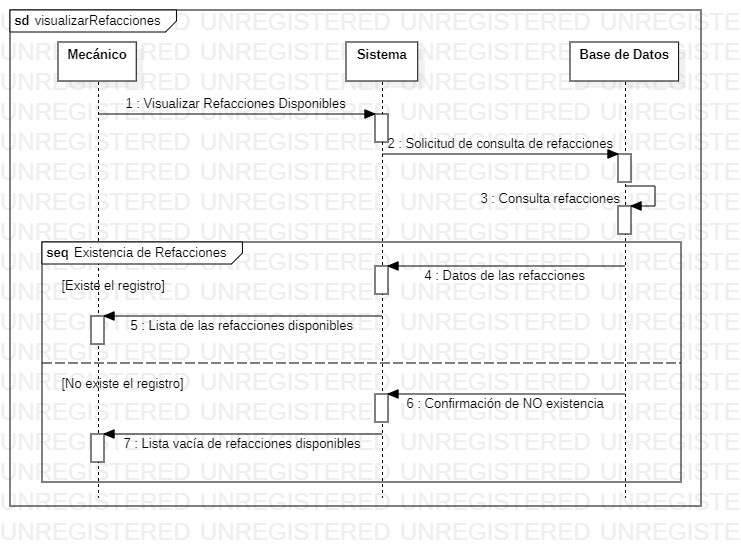
\includegraphics[width=0.8\textwidth]{./diseno/vescenarios/imagenes/visualizarRefacciones}
	\caption{Pantalla Visualizar Refacciones Admin (Búsqueda) - Vista de Escenarios}
	\label{fig:Pantalla refacciones busqueda- Vista de Escenarios}
\end{figure}
\clearpage